\subsection{Lagrangian's equations for a single particle}
\label{ap:particles_eq}


We now introduce an additional property of the particles: the total energy $E_\alpha$, which is defined as
\begin{equation*}    
    m_\alpha E_\alpha(t) 
    = \intO{ \rho_d [e_d^0 + (u_d^0)^2/2] }
    % + \intS{ \gamma },
\end{equation*}
Using the decomposition $\textbf{u}_d^0 = \textbf{u}_\alpha + \textbf{w}_d^0$, the total energy $E_\alpha$ can be decomposed according to,
\begin{equation*}
    \label{eq:E_alpha_def}
    m_\alpha E_\alpha
    = m_\alpha e_\alpha 
    + W_\alpha
    + m_\alpha (u_\alpha)^2/2
    % + \gamma s_\alpha 
\end{equation*}
Consequently, the total energy of a particle is the contribution of :
its internal energy $m_\alpha e_\alpha$; 
its internal kinetic energy, $W_\alpha =  \intO{\rho_d  (w_d^0)^2/2 }$;
its center of mass kinetic energy, $u_\alpha^2/2$;. 
Finally, we introduce the total energy of both the volume and the surface of the particle, which is defined as 
\begin{equation*}
    m_\alpha E_\alpha^\text{tot}
    = 
    \frac{s_\alpha}{m_\alpha} \gamma 
    + m_\alpha E_\alpha
\end{equation*}
where we noted $s_\alpha = \intS{}$ the surface of the particle $\alpha$, thus  $\gamma s_\alpha $ corresponds to the surface energy of the particle. 


\subsubsection{First order law}

Using the local conservation, \ref{eq:dt_rho}, \ref{eq:dt_rhou_k} and \ref{eq:dt_rhoE_k} into the generic formulation \ref{eq:dt_q_alpha} yields directly the mass momentum and total energy conservation equation for a single particle, namely
\begin{align}
    \ddt m_\alpha
    &= 
    0,\\
    \ddt (m_\alpha \textbf{u}_\alpha)
    &= 
    m_\alpha\textbf{g}
    +  \intS{\bm{\sigma}_d^0 \cdot \textbf{n}_d},\\
    \ddt (m_\alpha E_\alpha)
    &= 
    m_\alpha \textbf{u}_\alpha \cdot \textbf{g}
    +\intS{\textbf{u}_d^0 \cdot \bm{\sigma}_d^0 \cdot  \textbf{n}_d} 
    - \intS{\textbf{q}_d^0 \cdot \textbf{n}_d}. 
\end{align}
As mentioned in \ref{sec:Lagrangian} we now need to derive the particle's surface equations to re-formulate the exchange terms on the right-hand side of these equations. 
It is done by integrating \ref{eq:surface_tension}, \ref{eq:dt_rhoI_uI3} and  \ref{eq:dt_rhoIe_I}  over the surface of the particle, which gives,  
\begin{align}
    \label{eq:int_u_I}
    \intS{\Jump{\bm{\sigma}_k^0} }
    &=
    \intS{\divI\bm\sigma^0_{I||}} = 0\\
    \label{eq:int_u_I2}
    \intS{\Jump{\textbf{u}_k^0 \cdot \bm{\sigma}_k^0}},
    % = \intS{\Jump{\textbf{w}_k^0 \cdot \bm{\sigma}_k^0}},
    &=
    -\intS{\gamma(\textbf{n}\cdot \textbf{u}_{I}^0)(\div \textbf{n})}
    = \gamma \ddt s_\alpha,\\
    \label{eq:int_q_I}
    \Jump{\textbf{q}_k^0}
    &=
    0,
\end{align}
respectively. 
The second equality of \ref{eq:int_u_I} is demonstrated using \ref{eq:gauss_surface}. 
The second equality of \ref{eq:int_u_I2} is derived using both \ref{eq:gauss_surface} and \ref{eq:reynolds_transport}. 
As witnesses by \ref{eq:int_u_I}, on a closed surface the surface tension plays no role in the momentum jump condition.
Additionally, according to \ref{eq:int_u_I2} the work of the surface tension force is equal to $\gamma$ times the rate of change of the area of a given particle. 

Using \ref{eq:int_u_I}, \ref{eq:int_u_I2} and \ref{eq:int_q_I} to reformulate the preceding equations, we easily derive the total mass, momentum and energy equations for a single particle, 
\begin{align}
    \label{eq:dt_m_alpha}
    \ddt m_\alpha
    &= 
    0\\
    \label{eq:dt_p_alpha}
    \ddt (m_\alpha \textbf{u}_\alpha)
    &= 
    m_\alpha\textbf{g}
    +  \intS{\bm{\sigma}_f^0 \cdot \textbf{n}_d}\\
    \label{eq:dt_E_alpha_tot}
    \ddt (m_\alpha E_\alpha^\text{tot})
    &= 
    m_\alpha \textbf{u}_\alpha \cdot \textbf{g}
    +\textbf{u}_\alpha \cdot \intS{\bm{\sigma}_f^0 \cdot \textbf{n}_d}
    +\intS{\textbf{w}_f^0 \cdot \bm{\sigma}_f^0 \cdot  \textbf{n}_d} 
    - \intS{\textbf{q}_f^0 \cdot \textbf{n}_d}
\end{align}
where  $\intS{  \bm{\sigma}_f^0 \cdot \textbf{n}_d }$ is the resultants of the hydrodynamic force of the continuous phase, $\intS{\textbf{w}_f^0 \cdot \bm{\sigma}_f^0 \cdot  \textbf{n}_d} $ is the resultant of the work of the continuous phase stresses with the surface velocity, and $\intS{ \textbf{q}_f^0 \cdot \textbf{n}_d }$ is the resultants of the surface heat flux. 
Notice that the second term on the right hands side of \ref{eq:dt_E_alpha_tot} is the work produced by the mean force and the translational motion of the droplets, while $\intS{\textbf{w}_f^0 \cdot \bm{\sigma}_f^0 \cdot  \textbf{n}_d}$ is the work produced by the local forces and local motion of the fluid at the surface of the particle.
Note that these equations does not explicitly account for inter-particle interactions. 
Nevertheless, note that the surface external stress flux $\bm{\sigma}_f^0$ contains inter-particle forces mediated through the carrier fluid such as lubrication forces and long range inter-particle forces.

In the spirit of the energy decomposition exposed in the previous section (\ref{eq:dt_rhou_k2} and \ref{eq:dt_rhoe_k} )the total energy equation \ref{eq:dt_E_alpha_tot} can be split into three secondary equations. 
One for the center of mass kinetic energy $u_\alpha^2/2$, another for the particle internal kinetic energy $W_\alpha$, and a last one for the particle internal energy $e_\alpha$, it reads
\begin{align}
    \label{eq:dt_u2_alpha}
    \frac{1}{2}\ddt (m_\alpha u_\alpha^2)
    &= 
    \textbf{u}_\alpha\cdot
    \textbf{g}m_\alpha
    + 
    \textbf{u}_\alpha\cdot
    \intS{\bm\sigma_f^0 \cdot \textbf{n}_d},\\
    \label{eq:dt_w2_alpha}
    \ddt (W_\alpha + \gamma s_\alpha)
    &= 
    - \intO{ \bm{\sigma}_d^0 : \grad\textbf{u}_d^0 }
    + \intS {\textbf{w}_f^0 \cdot \bm{\sigma}_f^0 \cdot \textbf{n}_d }
    \\
     \label{eq:dt_e_alpha}
    \ddt (m_\alpha e_\alpha )
    &= 
     \intO{ \bm{\sigma}_d^0 : \grad\textbf{u}_d^0  }
    -  \intS{\textbf{q}_f^0\cdot \textbf{n}_d } 
\end{align}
respectively. 
The first equation is obtained by taking the dot product of \ref{eq:dt_p_alpha} with $\textbf{u}_\alpha$. 
The third equation is directly obtained using the local conservation of $e_k^0$ (\ref{eq:dt_rhoe_k}) and setting $f_d^0 = e_d^0$ in \ref{eq:dt_q_alpha_tot}.
The last equation is obtained by subtracting the first and third equations to \ref{eq:dt_E_alpha_tot}. 
Note that under this form the surface energy plays the role as a spring in the energy balance.   
From this set of equation we can easily see that the rate of dissipation terms $\intS{\bm{\sigma}_d^0 : \grad\textbf{u}_d^0}$ represent an energy sink in the equation of $W_\alpha$ while it is a source term in the internal energy equation. 
As it has been observed in the previous section, this terms convert the energy of internal motion to molecular agitation. 
However, the interplay between the center of mass  kinetic energy and the internal fluctuation is not obvious, indeed \ref{eq:dt_u2_alpha} shears no common term with the heat and internal kinetic energy equation.
In fact, we will see that the transfer between these scales is archived thought the fluid phase pseudo turbulent energy. 



\subsubsection{Higher moments balance}

In the objective of describing the shape as well as the deformation of a particle we now introduce the second moment of mass and first order moment of momentum of a particle. 
Following \ref{eq:Q_n_definition} we define the second-order moment of mass and the first-order moment of momentum as respectively,
\begin{equation}
    \textbf{M}_\alpha 
    = \intO{ \rho_d \textbf{r} \textbf{r} }
    \;\;\;\text{and}\;\;\;
    \textbf{P}_\alpha 
    = \intO{ \rho_d \textbf{r} \textbf{u}_d^0 }.
    \label{eq:first_moment_of_momentum_def}
\end{equation}
Note that $\textbf{M}_\alpha$ is analogous to the inertia tensor $\textbf{I}_\alpha$ in solid mechanics, both are related through the expression $\textbf{I}_\alpha = \bm\delta : \textbf{M}_\alpha - \textbf{M}_\alpha$.
For a constant density, the tensor $\textbf{M}_\alpha$ describes the second moment of the volume distribution around the particle center of mass.
Likewise, the tensor $\textbf{P}_\alpha$ describes the first moment of the velocity distribution within the particle volume. 
To provide a clearer physical interpretation of the moment of momentum tensor, we decompose $\textbf{P}_\alpha$ into two distinct parts. 
Namely, 
$\textbf{P}_\alpha = \textbf{S}_\alpha+\textbf{T}_\alpha$, where $\textbf{S}_\alpha$ represents the symmetric part and $\textbf{T}_\alpha$ is the antisymmetric part of $\textbf{P}_\alpha$.
Then, the tensors $\textbf{S}_\alpha$ and $\textbf{T}_\alpha$ correspond respectively to the stretching and angular momentum of the particle $\alpha$. 
The tensor $\textbf{S}_\alpha$ quantifies how fast and in which direction the particle gets elongated or flattened, in other words it represents the mean rate of deformation experienced by the particle.
The tensor $\textbf{T}_\alpha$ is related to the angular momentum of the particle denoted by the pseudo vector $\bm\mu_\alpha = \intO{ \rho_d \textbf{r} \times \textbf{u}_d^0 }$. 
Indeed, both  $\textbf{T}_\alpha$ and $\bm{\mu}_\alpha$ represent the angular momentum and are related through $(\bm{\mu}_\alpha)_i = \epsilon_{ijk} (\textbf{P}_\alpha)_{jk}= \epsilon_{ijk} (\textbf{T}_\alpha)_{jk}$, where $\bm\epsilon$ is the third order alternating unit tensor or Levi-Cita tensor. 
Lastly, we also introduce the scalar $M_\alpha =\frac{1}{3}\bm\delta : \textbf{P}_\alpha = \frac{1}{3}\intO{ \rho_d \textbf{r} \cdot \textbf{u}_d^0 }.$, which quantifies the rate at which the particle is being compressed or expanded.
To better explain the implication of these quantities on the particle kinematics we provide in \ref{eq:scheme}, three schemes representing possible inner velocity fields with their corresponding value of the moment of momentum tensor.
Note that in \ref{eq:scheme} we explicit
\begin{figure}[h!]
    \centering
    \hfill
    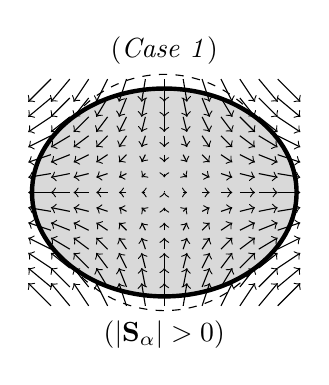
\begin{tikzpicture}[ultra thick,scale=0.6]
        \def\nRows{6}
        \def\nCols{6}
        \draw[dashed,thin] (0,0)circle(2.5);
        \draw[fill=gray!30] (0,0)ellipse(2.8 and 2.2);
        \foreach \x in {-\nRows,...,\nRows} {
            \foreach \y in {-\nCols,...,\nCols} {
                \pgfmathsetmacro\distance{veclen(\x*0.4, \y*0.4)};
                \pgfmathparse{\distance < 2.45 ? "blue" : "white"}
                \edef\colour{\pgfmathresult};
                \ifthenelse{\equal{\colour}{blue}}{                    
                    \draw[thin,->](\x*0.4,\y*0.4)--++(0.08*\x,-0.08*\y);
                }
            }
        }
        \node (txt) at (0,3){(\textit{Case 1})};
        \node (txt) at (0,-3){($|\textbf{S}_\alpha| > 0$)};
    \end{tikzpicture}
     \hfill
    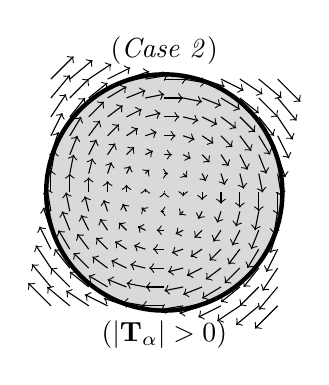
\begin{tikzpicture}[ultra thick,scale=0.6]
        \def\nRows{6}
        \def\nCols{6}
        \draw[fill=gray!30] (0,0)circle(2.5);
        \foreach \x in {-\nRows,...,\nRows} {
            \foreach \y in {-\nCols,...,\nCols} {
                \pgfmathsetmacro\distance{veclen(\x*0.4, \y*0.4)};
                \pgfmathparse{\distance < 2.5 ? "blue" : "white"}
                \edef\colour{\pgfmathresult};
                \ifthenelse{\equal{\colour}{blue}}{                    
                    \draw[thin,->](\x*0.4,\y*0.4)--++(0.08*\y,-0.08*\x);
                }
            }
        }
        \node (txt) at (0,3){(\textit{Case 2})};
        \node (txt) at (0,-3){($|\textbf{T}_\alpha| > 0$)};
    \end{tikzpicture}
    \hfill
    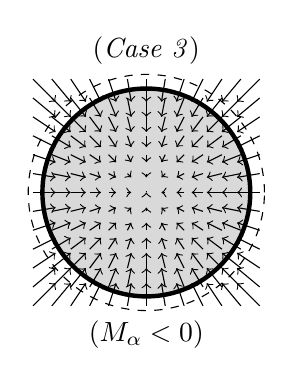
\begin{tikzpicture}[ultra thick,scale=0.6]
        \def\nRows{6}
        \def\nCols{6}
        \draw[dashed,thin] (0,0)circle(2.5);
        \draw[fill=gray!30] (0,0)circle(2.2);
        \foreach \x in {-\nRows,...,\nRows} {
            \foreach \y in {-\nCols,...,\nCols} {
                \pgfmathsetmacro\distance{veclen(\x*0.4, \y*0.4)};
                \pgfmathparse{\distance < 2.3 ? "blue" : "white"}
                \edef\colour{\pgfmathresult};
                \ifthenelse{\equal{\colour}{blue}}{                    
                    \draw[thin,->](\x*0.4,\y*0.4)--++(-0.08*\x,-0.08*\y);
                }
            }
        }
        \node (txt) at (0,3){(\textit{Case 3})};
        \node (txt) at (0,-3){($M_\alpha < 0$)};
    \end{tikzpicture}
    \hfill
    \caption{Graphical representation of the inner kinematics of an arbitrary particle under three scenarios. 
        The arrows represent the velocity field inside the particle, $\textbf{w}_d^0$, with the corresponding value of the moment of momentum tensor indicated below. 
        The operator $|\ldots|$ refers to the norm of the tensors. 
        According to the inner velocity field:
        (\textit{Case 1}) The particle experiences a mean rate of deformation, resulting in non-zero stretching of momentum along the principal axis of deformation;
        (\textit{Case 2}) The particle is rotating, leading to a non-zero angular momentum vector in the direction of rotation;
        (\textit{Case 3}) The particle undergoes compression, resulting in a negative trace of the moment of momentum.
    }
    \label{eq:scheme}
\end{figure}

Injecting, $f_d^0 = \rho_d$ in the second-order moment equation (derived in \ref{ap:Moments_equations}) we obtain :
\begin{equation}
    \ddt {\textbf{M}_\alpha}=2\textbf{S}_\alpha. 
    \label{eq:dt_M_alpha}
\end{equation}
which is the second-order moment of mass conservation equation. 
From \ref{eq:dt_M_alpha} we deduce that the evolution of the distribution of mass of a particle is solely motivated by the stretching of momentum $\textbf{S}_\alpha$. 
This implies that the angular momentum (not to be confused with the angular velocity) plays no role in the evolution of the second moment of mass. 
This is due to the symmetry of the tensor $\textbf{M}_\alpha$, which must be preserved after differentiation with respect to time.
Note that if the particle has a constant $\textbf{M}_\alpha$ under change of reference frame, such as for spherical particles where we can write $\textbf{M}_\alpha= \frac{a^2 m_\alpha}{5} \bm\delta$, then $\textbf{S}_\alpha=0$ since $\ddt \textbf{M}_\alpha = 0$ in this situation.
This argument has no restriction on the internal particle motions, thus it is also true for fluid particles with possible inner motion. 
Additionally, applying the trace operator on both sides of \ref{eq:dt_M_alpha}, yields the interesting relation $\ddt {M_\alpha}=\frac{2}{3}\bm\delta : \textbf{S}_\alpha$.
We can state that $M_\alpha = \lambda^\alpha_f(t)+\lambda^\alpha_d(t)+\lambda^\alpha_3(t)$, with $\lambda_i^\alpha$ for $i=1,2,3$, the eigenvalues of $\textbf{M}_\alpha$, as it is a symmetric tensor and thus always diagonalizable.
For undeformable particles, it is evident that the eigenvalues are not functions of time, implying $\ddt M_\alpha = 0$.  
Consequently, $\bm\delta : \textbf{S}_\alpha$ possesses the notable property of being zero whenever the particle shape remains constant, regardless of the orientation.

Now that we have described the kinematics of the particle shape, let us proceed to derive an equation for the dynamics of the particle shape, i.e. an equation for the moment of momentum. 
This equation is derived injecting $\textbf{Q}_\alpha = \textbf{P}_\alpha$ in \ref{eq:dt_Q_alpha_tot}, it reads, 
\begin{equation}
    \ddt {\textbf{P}_\alpha}
    - \intO{ \rho_d  \textbf{w}_d^0 \textbf{w}_d^0 }
    = 
    - \intO{\bm{\sigma}_d^0}
    - \intS{ 
        \gamma (\bm\delta - \textbf{nn})
    }
    + \intS{ \textbf{r}\bm{\sigma}_f^0\cdot \textbf{n}_d}.
    \label{eq:dt_P_alpha}
\end{equation}
On the left-hands side of \ref{eq:dt_P_alpha} we identify two inertial terms, i.e. the derivative of $\textbf{P}_\alpha$ and the internal velocity term $\intO{\rho_d\textbf{w}_d^0\textbf{w}_d^0 }$.
The inertia of the particle is then balanced by the terms on the right-hand side of the equation, namely: 
the integral of the particle internal stress $\intO{ \bm{\sigma}_d^0}$; 
the integral of the surface tension stress $\intS{ \gamma (\bm\delta- \textbf{nn}) }$; 
and the first moment of the hydrodynamic stress tensor, $\intS{\textbf{r}\bm\sigma_f^0\cdot \textbf{n}}$.
A discussion regarding the physical implications of this equation is provided below. 

The conservation equation of the angular momentum $\bm{\mu}_\alpha$ is obtained by taking the double contracted product of \ref{eq:dt_P_alpha} with $\bm\epsilon$, which gives 
\begin{equation}
    \ddt\bm{\mu}_\alpha
    =  
    % \textbf{t}_\alpha.
    \intS{ \textbf{r} \times \bm{\sigma}_f^0\cdot \textbf{n}_d }
    \label{eq:dt_mu_alpha}
\end{equation}
Notice that every term on the right-hand side of \ref{eq:dt_P_alpha} vanished due to their symmetric nature apart from the shew-symmetric part of the hydrodynamic stress, which is the hydrodynamic torque applied on the particle $\alpha$.
Particularly, the surface tension terms do not appear in the angular momentum balance since $\bm\sigma_I^0 = \gamma (\bm\delta-\textbf{nn})$ is symmetric, which is consistent with the findings of \citet{hesla1993note}. 
As a consequence, the surface tension does not affect the angular momentum regardless of the particle's shape. 
In the literature, it is common to include the torque due to inter-particular interactions in the angular momentum balance, as is done in \citet{jackson1997locally} and \citet{zhang1997momentum}.
In our case note that $\bm{\sigma}_f^0$ contains also short-range interaction forces which can be assimilated to the particle-particle interaction forces.

Taking the double contracted product of \ref{eq:dt_P_alpha} with the tensor $\bm\delta$ and using \ref{eq:dt_M_alpha}, yields directly  
% \begin{equation}
%     \frac{1}{2}\ddt^2 {M_\alpha}
%     - \frac{1}{3}\intO{ \rho_d \textbf{w}_d^0 \cdot \textbf{w}_d^0}
%     = 
%     \intO{p_d^0} 
%     % - \frac{1}{3}\intS{p_f^0 \textbf{r}\cdot \textbf{n}}
%     - \frac{2}{3} \gamma s_\alpha
%     - \frac{1}{3}\intS{p_f^0 \textbf{r}\cdot \textbf{n}}
%     + \frac{1}{3}\intS{\textbf{r}\cdot\bm\tau_f^0\cdot \textbf{n}},
%     \label{eq:dt_D_alpha}
% \end{equation}
\begin{equation}
    \frac{3}{2}\frac{d^2 M_\alpha}{dt^2}
    - \intO{ \rho_d \textbf{w}_d^0 \cdot \textbf{w}_d^0}
    = 
    - \intO{\bm\sigma_d^0:\bm\delta} 
    % - \frac{1}{3}\intS{p_f^0 \textbf{r}\cdot \textbf{n}}
    - \gamma 2 \intS{}
    % - \frac{1}{3}\intS{p_f^0 \textbf{r}\cdot \textbf{n}}
    + \intS{\textbf{r}\cdot\bm\sigma_f^0\cdot \textbf{n}}.
    \label{eq:dt_D_alpha}
\end{equation}
\ref{eq:dt_D_alpha}, corresponds to the isotropic work balance over the volume and surface of the particle. 
According to \ref{eq:dt_D_alpha}, the rate of compression of a particle, denoted by the second derivative of $M_\alpha$ evolves according to : 
the internal inertial term, $\intO{\rho_d \textbf{w}_d^0 \cdot \textbf{w}_d^0 }$;
the particle internal pressure $\intO{\bm\sigma_d^0:\bm\delta}$; 
the surface energy $\gamma\intS{  }$; 
and the trace of the hydrodynamic first moment $\intS{\textbf{r}\cdot\bm\sigma_f^0\cdot \textbf{n}}$.
If one considers spherical particles composed of compressible fluid, \ref{eq:dt_D_alpha} transforms into the Rayleigh-Lamb-Plesset equation. 
In the steady-state regime, this reduces to the Young-Laplace equation, as indicated by the presence of the first three terms on the right-hand side of \ref{eq:dt_D_alpha}. 

% \tb{
%     As an example we now consider the \textit{Rayleigh-Lamb-Plesset} equation for spherical bubbles with radius $a_\alpha(t)$. 
%     As the droplets remain spherical while keeping a constant mass the moment of momentum and inner velocity field can be expressed, 
%     \begin{align*}
%         M_\alpha
%         = \frac{m_\alpha}{5} a^2_\alpha(t),
%         && 
%         \textbf{w}_d^0
%         = \frac{d a_\alpha}{dt}\frac{\textbf{r}}{a_\alpha(t)},
%         \label{eq:expr1}
%     \end{align*}
%     where it is empathized that the radius $a_\alpha(t)$ is time-dependent. 
%     The stress inside the bubbles might be expressed as compressible Newtonian fluids with no resistance to shear such that 
%     \begin{equation}
%         \bm\sigma_d^0 
%         = 
%         - p_d^0 \bm\delta
%         - \lambda_d (\div \textbf{u}_d^0) \bm\delta
%         % + \mu_d \left[\grad \textbf{u}_d^0 + (\grad \textbf{u}_d^0)^\dagger\right]
%         = 
%         - p_d^0 \bm\delta
%         - \frac{3 \lambda_d}{a_\alpha} \frac{d a_\alpha}{dt}  \bm\delta
%         % + \mu_d \left[\grad \textbf{u}_d^0 + (\grad \textbf{u}_d^0)^\dagger\right]
%         \label{eq:StressBubbles}
%     \end{equation}
%     where $\lambda_d^0$ is the volume viscosity of the dispersed phase. 
%     Assuming incompressible Newtonian fluid for the continuous phase and injecting the expressions \ref{eq:StressBubbles} and \ref{eq:expr1} into \ref{eq:dt_D_alpha} yields, 
%     \begin{equation}
%         \frac{1}{5} \rho_d^0 a_\alpha \frac{d^2 a_\alpha}{dt^2} 
%         - 
%         \frac{1}{a_\alpha} \frac{d a_\alpha}{dt} 
%         \left(
%             3 \lambda_d
%             + 2 \mu_f 
%         \right)
%         = 
%         +  \frac{1}{v_\alpha}\intO{p_d^0}
%         -  \frac{1}{s_\alpha}\intS{p_f^0}
%         - \gamma  \frac{2}{a}
%     \end{equation}
%     By expressing the fluid pressure on the surface in terms of the far field pressure (see daniel) one obtain the \textit{Rayleigh-Lamb-Plesset} equation. 
%     In the static regime we recover laplace eq
% }

Taking the symmetric part of \ref{eq:dt_P_alpha}, and making use of \ref{eq:dt_M_alpha}, yields a dynamical balance equation for $\textbf{M}_\alpha$, namely
% \begin{multline}    
%     \frac{1}{2}\ddt^2{\textbf{M}_\alpha^\text{dev}}
%     - \intO{\left(
%         \rho_d\textbf{w}_d^0 \textbf{w}_d^0
%         - \rho_d\frac{1}{3}(\textbf{w}_d^0 \cdot \textbf{w}_d^0)\bm\delta\right)}
%     =  
%         - \mu_d \intO{\textbf{e}_d^0}
%         - \intS{\gamma\left(\frac{1}{3}\bm\delta-\textbf{nn}\right)}\\
%         + \frac{1}{2}\intS{\left(\textbf{r}\bm\sigma_f^0+ \bm\sigma_f^0\textbf{r} - \frac{2}{3}(\bm\sigma_f^0\cdot \textbf{r})\bm\delta\right)\cdot \textbf{n}}
%     \label{eq:dt_S_alpha}
% \end{multline}
\begin{equation}    
    \frac{1}{2}\frac{d^2 \textbf{M}_\alpha}{dt^2}
    - \intO{ \rho_d  \textbf{w}_d^0 \textbf{w}_d^0 }
    = 
    - \intO{\bm{\sigma}_d^0}
    - \intS{\gamma (\bm\delta - \textbf{nn})}
    + \frac{1}{2}\intS{(\textbf{r}\bm{\sigma}_f^0+\bm{\sigma}_f^0 \textbf{r})\cdot \textbf{n}_d}.
    \label{eq:dt_S_alpha}
\end{equation}
On the left-hand side of \ref{eq:dt_S_alpha}, we recover the symmetric part of the inertial contributions. 
Especially, in opposition to \ref{eq:dt_P_alpha} we could substitute $\textbf{P}_\alpha+\textbf{P}_\alpha^\dagger$ by $\ddt \textbf{M}_\alpha$. 
Consequently, \ref{eq:dt_S_alpha} is a dynamical equation for the droplet mean deformation. 
In our case, only the external contribution $\frac{1}{2}\intS{\textbf{r}\bm\sigma_f^0\cdot \textbf{n}}$ is responsible for the generation of angular momentum, see \ref{eq:dt_mu_alpha}.
Taking the symmetric part of this tensor ultimately removes this contribution. 
Thus, on the right-hand side of \ref{eq:dt_S_alpha}, we identify the terms responsible for the droplet deformation exclusively.
Therefore, \ref{eq:dt_S_alpha} must be interpreted as an equation for the shape of the particle, represented by the tensor $\textbf{M}_\alpha$.

One might immediately recognize that this equation is in fact an extension of Batchelor’s famous result, 
\begin{equation}
    \intO{\bm{\sigma}_d^0}
    + \intS{\gamma(\bm\delta - \textbf{nn})}
    = \frac{1}{2}\intS{(\textbf{r}\bm\sigma_f^0+\bm\sigma_f^0\textbf{r})\cdot \textbf{n}},
    \label{eq:Batchelor}
\end{equation}
but with the consideration of the inertia of the particle.
\ref{eq:Batchelor} is particularly useful to express the unknown internal stress within solid particles (in which case $\gamma = 0$), in terms of surface integral, i.e. the stresslet $\intS{(\textbf{r}\bm\sigma_d^0+ \bm\sigma_d^0\textbf{r})\cdot \textbf{n}}$.
This relation is the main tool used to express the bulk stress of a suspension, it eventually leads to the computation of the famous Einstein equivalent viscosity, upon having a closed expression for the average of $\intS{(\textbf{r}\bm\sigma_d^0+ \bm\sigma_d^0\textbf{r})\cdot \textbf{n}}$ \citep{guazzelli2011}. 
In the inertial case, due to the limited degree of freedom of solid particles, the tensors $\textbf{M}_\alpha$ and the inner velocity field $\textbf{w}_d^0$ are fully determined by \ref{eq:dt_M_alpha} and \ref{eq:dt_mu_alpha}, indicating that $\textbf{M}_\alpha$ and $\textbf{w}_d^0$ can be utilized in \ref{eq:dt_S_alpha} not as unknowns but as source terms. 
Consequently, for solid particles, \ref{eq:dt_S_alpha} must be interpreted as a generalized equation for the undefined stress $\bm\sigma_d^0$ integrated on the volume of the particles.
Whether it is solid or fluid particles \ref{eq:dt_S_alpha} becomes particularly relevant for expressing the averaged stress within an inertial suspension in terms of Lagrangian properties, as discussed in section \ref{sec:averaged_eq}.

It is now clear that if the surface tension forces play no role in the linear and angular momentum equation, it does impact the moment of momentum $\textbf{P}_\alpha$ or more specifically its symmetric part $\textbf{S}_\alpha$.
Thus, the surface tension force impacts the hydrodynamic behavior of a particle solely through its action on $\textbf{S}_\alpha$, which is related to the shape of a particle represented by $\textbf{M}_\alpha$, through \ref{eq:dt_M_alpha}.
In \ref{ap:Moments_equations} we show how to derive the higher-order moment of momentum equations, which can also be viewed as formulas for the higher moments of the internal particle stress distribution. 
It is interesting to mention that in a recent study of \citet{dolata2021faxen} and \citet{zhou2020lamb} they use energy methods and recover the first two moments of momentum equations hidden into another but equivalent form, valid in the Stokes flow regime. 

Hence, the moment of momentum emerges as a quantity of utmost importance for all types of particles with variable shape or volume. 

